\documentclass[11pt]{article}
\usepackage{amsmath, amssymb}
\usepackage{geometry}
\geometry{margin=1in}
\usepackage{fancyhdr}
\usepackage{lastpage}
\usepackage{parskip} % Better paragraph spacing
\usepackage{titlesec} % Better section formatting
\usepackage{graphicx}
\usepackage{float}
\usepackage[most]{tcolorbox}
\usepackage{lmodern}
\usepackage{caption}
\usepackage{hyperref}
\usepackage{listings}
\usepackage{xcolor}

\definecolor{codegreen}{rgb}{0,0.6,0}
\definecolor{codegray}{rgb}{0.5,0.5,0.5}
\definecolor{codepurple}{rgb}{0.58,0,0.82}
\definecolor{backcolour}{rgb}{0.95,0.95,0.92}

% Define code styling
\lstdefinestyle{mystyle}{
    backgroundcolor=\color{backcolour},
    commentstyle=\color{codegreen},
    keywordstyle=\color{magenta},
    numberstyle=\tiny\color{codegray},
    stringstyle=\color{codepurple},
    basicstyle=\ttfamily\footnotesize,
    breakatwhitespace=false,
    breaklines=true,
    captionpos=b,
    keepspaces=true,
    numbers=left,
    numbersep=5pt,
    showspaces=false,
    showstringspaces=false,
    showtabs=false,
    tabsize=2
}

\lstset{style=mystyle}

% Define commands for reusable content
\newcommand{\coursename}{COM-402 Information Security and Privacy}
\newcommand{\lecturenum}{11}
\newcommand{\lecturedate}{\today}
\newcommand{\professor}{Mathias Payer}

\hypersetup{colorlinks=true,linkcolor=blue,urlcolor=blue}

% Configure section spacing
\titlespacing*{\section}{0pt}{2ex plus 1ex minus .2ex}{1.5ex plus .2ex}
\titlespacing*{\subsection}{0pt}{1.5ex plus 1ex minus .2ex}{1ex plus .2ex}
% Header / Footer
\pagestyle{fancy}
\fancyhf{}
\fancyhead[L]{\coursename}
\fancyhead[R]{Lecture \lecturenum}
\fancyfoot[L]{EPFL - Computer Science}
\fancyfoot[C]{Author: Jonathan Dutoit}
\fancyfoot[R]{Page \thepage\ of \pageref{LastPage}}

\begin{document}

\begin{center}
  {\large EPFL - Computer Science} \\[0.5em]
  {\Large \textbf{\coursename}} \\[0.5em]
  {\large Lecture \lecturenum\ --- \lecturedate} \\[0.5em]
  {\large Author: Jonathan Dutoit} \\[0.5em]
  {\large Professor: \professor} \\[0.5em]
\end{center}

\vspace{2cm}

\begin{center}
  {\LARGE \textbf{Privacy}}
\end{center}

\vspace{1cm}

\section*{Learning goals}
\begin{itemize}
	\item Privacy is not about hiding, privacy is about preventing harm
	\item Privacy has many definitions: know your goal and adversary
	\item Where we need privacy: when designing privacy-preserving systems
	\item A good privacy evaluation requires good threat modeling
	\item Some example of Privacy Enhancing Technologies
\end{itemize}

\textbf{Disclaimer}: you will not become a privacy engineer today. This is a very light introduction.

\section*{Outline}

\begin{itemize}
	\item Why privacy matters
	\item What is privacy: two angles relevant for privacy engineering
	\item Building privacy-preserving systems
	\item Example of PETS and their evaluation
	\item The quest for anonymization and pitfalls
	\begin{itemize}
		\item K-anonymity
	\item Query auditing
	\item Differential privacy 
\end{itemize}
	
\end{itemize}

\newpage

\begin{center}
  {\LARGE \textbf{Why Privacy Matters}}
\end{center}
\vspace{0.5cm}

Privacy is default by law:

\begin{tcolorbox}[
  colback=gray!15,     % background color
  colframe=black!50,    % border color
  boxrule=1pt,       % border thickness
  arc=3mm,             % rounded corners
  left=4mm, right=4mm, top=2mm, bottom=2mm % padding
]
\textbf{Article 12}

\vspace{0.3cm}

No one shall be subjected to arbitrary interference with his privacy, family, home or correspondence, nor to attacks upon his honour and reputation. Everyone has the right to the protection of the law against such interference or attacks.
\end{tcolorbox}

But, in our digital society: many online services collect private data. Thin line between the usefulness of information and data collected.

\textbf{So what if they know...?} I have nothing to hide!

\section*{Target(ed) advertising}

Target (fancy retailed in the USA - like "Globus") knows what you buy, when you buy it, how often, ...

Target can buy data (from 3rd party brokers) about you:
\begin{itemize}
	\item \textbf{Online}: what websites you visit, how long, in which order, what kinds of topics you search for online, what you like, what you share, ...
	\item \textbf{Offline}: your ethnicity, job history, the magazines you read, if you've ever declared bankruptcy or got divorced, the year you bought your house, where you went to college, the number of cars you own, ....
\end{itemize}

Target can use this information for
\begin{itemize}
	\item Sending customers with kids catalogs of toys before Christmas
	\item Sending customers who buy swimsuits in April coupons for sunscreen in July and died books in December
\end{itemize}

All of this may bring surprises... "How target figured out a teen girl was pregnant before her father did" in Forbes journal...

Target advertising can also be used to discriminate. Of the 500 simulated users, each, \textbf{402} male users received the ad at least once, buy only \textbf{60} female users received the same ad at least once. 

\section*{Facebook / Cambridge Analytica (2016)}

Context: CA obtained 50M records from Facebook in 2013 through "survey" app that leaked friends' information as well as from the user answering the survey

CA created a system that can target voters based on psychological profile

Was used to target US voters in 2016 elections and UK voters in Brexit

\subsection*{Consequences}

"Brexit vote" and US presidential elections: two leading democracies, find themselves internally polarized. 

\subsection*{Attribute-based targeting}

Each Facebook user has assigned attributes
\begin{itemize}
	\item computed by Facebook
	\item based on Likes, 3rd-party browsing (tracking via "Like" button), etc
	\item bought form "Partner" companies (Data brokers)
\end{itemize}
$>$ 1200 well-defined attributes

$>$ 250k "loosely defined" attributes (from text-processing)

Advertiser select attributes, Facebook relevant ads. Facebook doesn't reveal user identities.

We should use \textbf{Privacy plugins!}

\subsection*{Attribute-based targeting: PII-based (Personal Identifying Information)}

Advertiser can bulk-upload a database (bough from data brokers, etc.) to Facebook, who tells how many users are present on the system, and allows to target them. 

% Quick centered image
\begin{figure}[H]
    \centering
    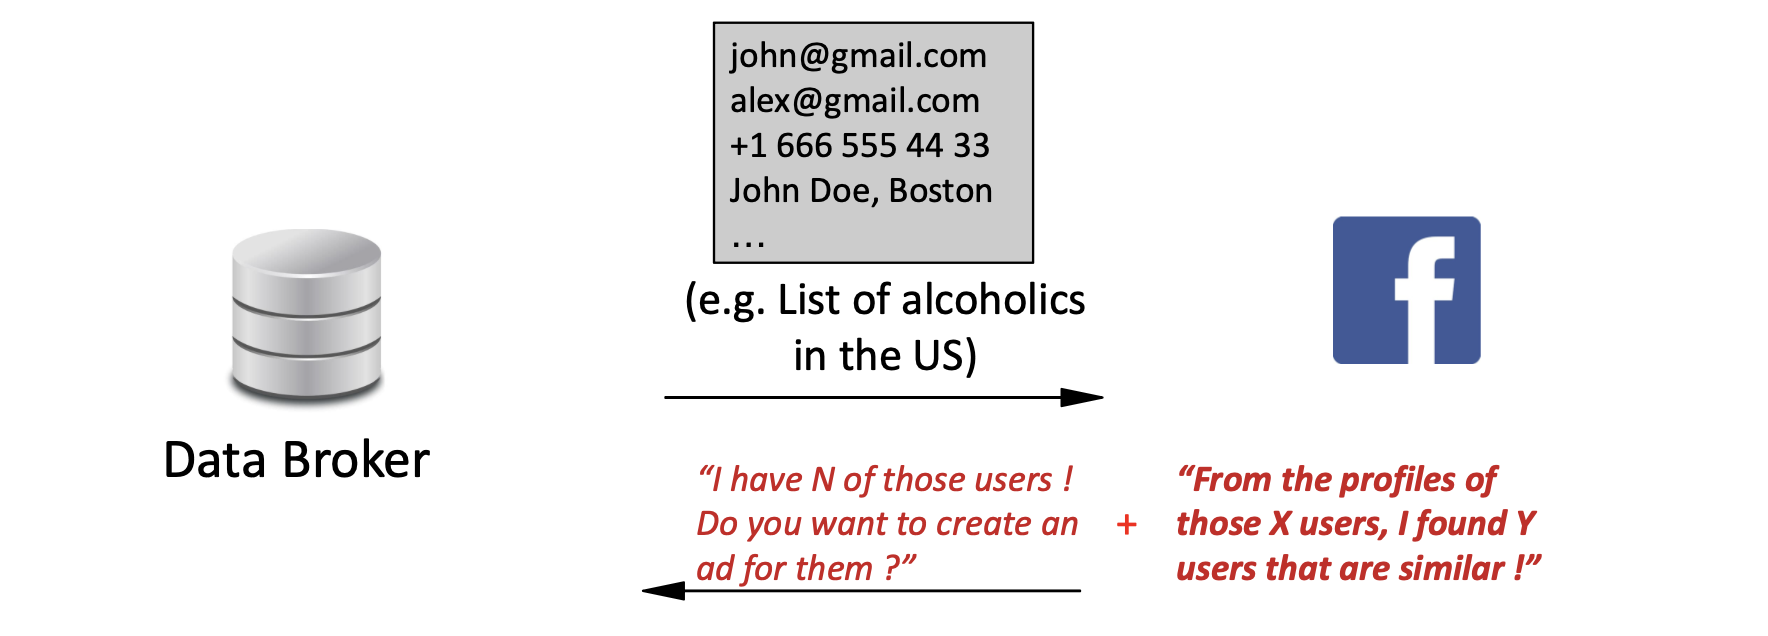
\includegraphics[width=0.8\textwidth]{databroker}
    \label{fig:LABEL}
\end{figure}

Facebook discovers "similar" people (that are not listed by Data Brokers) based on interests or browsing patterns. 

Can be tailored per region, sex, marital status and other attributes. 

\textbf{Not really ethical!}

\section*{2023 - EU Child Sexual Abuse (CSA) regulation debate}

\textbf{Very} controversial proposal 

REGULATION OF THE EUROPEAN PARLIAMENT AND OF THE COUNCIL laying down rules to prevent and combat child sexual abuse. 

"To sway European public opinion, however, the European Commission went even further. X’s Transparency Report shows that the European Commission also used ‘microtargeting’ to ensure that the ads did not appear to people who care about privacy (people interested in Julian Assange) and eurosceptics (people interested in ‘nexit’, ‘brexit’ and ‘spanexit’ or in Victor Orbán, Nigel Farage, or the German political party AfD).[17] For unclear reasons, people interested in Christianity were also excluded. After excluding critical political and religious groups, X’s algorithm was set to find people in the remaining population who were indeed interested in the ad message, resulting in an uncritical echo chamber. This microtargeting on political and religious beliefs violates X’s advertising policy,[18] the Digital Services Act[19] – which the Commission itself has to oversee – and the General Data Protection Regulation."

\section*{The privacy of whom?}

\textbf{Individuals}
\begin{itemize}
	\item protection against profiling and manipulation
	\item protection against crime / identity theft
\end{itemize}

Thus privacy is a security property -- there is no security without privacy

\textbf{Companies}
\begin{itemize}
	\item protection of trade secrets, business strategy, internal operations, ...
\end{itemize}
\textbf{Governments / military}
\begin{itemize}
	\item protection of national secrets, confidentiality of law enforcement investigations, diplomatic activities, political negotiations

\end{itemize}

\section*{Privacy must be for all}

\textcolor{red}{Denying privacy to some is denying privacy to all}

\textbf{INFRASTRUCTURE IS SHARED}

\textbf{Individuals, Industry, and Governments use the same applications!}

This can be done either \textbf{\textit{directly}} or \textbf{\textit{indirectly}}. Indirect example: Strava user for militaries in Africa base point out the military base map/schema by running around the military base. Disrupted operation due to secret information leakage. 

\section*{Security vs. Privacy - Common \textcolor{red}{Misconception}}

\textbf{We need tradeoff security for privacy!}

\begin{center}
	More surveillance implies more security which implies a safer world
\end{center}

\begin{itemize}
	\item Surveillance may be not \textbf{\underline{effective}}: smart adversaries evade surveillance
	\item Surveillance tools can be \underline{\textbf{abused}}; lack of transparency and safeguards
	\item Surveillance tools can be \textbf{\underline{subverted}} for crime / terrorism
\end{itemize}

\vspace{0.5cm}

\begin{center}
  {\LARGE \textbf{What is Privacy?}}
\end{center}
\vspace{0.5cm}

\section*{Defining privacy}

Privacy is subjective: hard to define

In this lecture: three ways of thinking about privacy depending on what goal are we trying to achieve: they are a way of reasoning about harm prevention

Different mindsets lead to different technologies - and different protection!

\section*{Privacy as Confidentiality}
“The right to be let alone” -Warren and Brandeis (1890)

"the individual shall have full protection in person and in property."

\begin{itemize}
	\item Goal: Minimize data disclosure (which includes distributing trust)
	\item PETS: encryption, privacy-preserving computation. Obfuscation, decentralization
		\begin{itemize}
			\item Homomorphic encryption, Secure Multiparty computation, Differential privacy
			\item Tor: anonymous communication network
		\end{itemize}
	\item Mathematical privacy definitions and strong proofs of security
\end{itemize}

\section*{Privacy as Control}
"“The claim of individuals, groups, or institutions to determine for themselves when, how, and to what extent information about them is communicated to others” - Westin (1970)
\begin{itemize}
	\item Goal: Let the user decide how data will be shared and used
	\item PETS: privacy settings, (automated) privacy policies, logging
		\begin{itemize}
			\item Secure logging, Sticky policies, ...
		\end{itemize}
	\item Organizational compliance and fines (GDPR, US Fair information principles)
\end{itemize}

\section*{Privacy as Practice}
"The freedom from unreasonable constrains on the construction of one's own identity" - Agre (1999)

\begin{itemize}
	\item Goal: Improve user agency with respect to private information
	\item PETS: contextual feedback, privacy nudges
\end{itemize}

\vspace{0.5cm}

\begin{center}
  {\LARGE \textbf{And because privacy is a security property... there is an adversary}}
\end{center}
\vspace{0.5cm}

\section*{Players/Adversaries}

\textbf{Social Context}
\begin{itemize}
	\item Colleagues
	\item Family and friends
	\item Strangers
\end{itemize}

\textbf{Institutional Adversaries}
\begin{itemize}
	\item Companies
	\item Advertisers
	\item Organizations we work for
\end{itemize}

\textbf{State-level / Global Adversaries}
\begin{itemize}
	\item Government
\end{itemize}

\subsection*{Adversaries from social context}

Concerns: problems from using technology
\begin{itemize}
	\item "My boss knows I am looking for another job"
\end{itemize}

PETs Goal: Do not surprise the user -- support decision making
\begin{itemize}
	\item \textbf{Easy defaults}
	\item \textbf{Contextual feedback}
	\item \textbf{Privacy nudges}
\end{itemize}

Limitations: only protects from other users, service provider is trusted!
\begin{itemize}
	\item Limited by user's capability to understand policies
	\item Based on user expectations, what if they are off?
\end{itemize}

\textbf{Snapchat have all of your photos!}

\subsection*{Many systems can be (stealthily) used for surveillance}

\textbf{Function creep:} expansion of a process or system where data collected for one specific purpose is subsequently used for another unintended or unauthorized purpose. 

\subsection*{A recurrent function \textit{creep} example: identity systems}
Aadhaar - India's "optional" Unique Identity identification number scheme 

$>$ 1 billion people stored in the database

\textbf{Goal}: \textit{promoted as providing the poor with an identity}

\textbf{It became:}
\begin{itemize}
	\item \textit{mandatory for opening a bank account}
	\item \textit{mandatory for benefits system}
	\item \textit{mandatory for buying a SIM card}
	\item \textit{required to pay taxes}
\end{itemize}


EURODAC - fingerprint database for asylum seekers

\textbf{Goal:}  store fingerprints from all people who cross the border into a European country without permission – asylum seekers as well as irregular migrants to help immigration and asylum authorities to better control irregular immigration to the EU, detect secondary movements (migrants moving from the country in which they first arrived to seek protection elsewhere) and facilitate their readmission and return to their countries of origin.

\textbf{It became:} database for police and public prosecutors, such as Europol. 

More data: in addition to fingerprints, the facial images and alphanumerical data (name, ID or passport number) of asylum seekers and irregular migrants will also be stored. 

\section*{Institutional adversaries}

Concerns: (defined by Legislation) data should not be collected without user \underline{consent} or processed for \underline{illegitimate uses}. Data should be secured: correct, integrity, deletion

PETs Goals: Compliance with data protection principles
\begin{itemize}
	\item Informed consent: valid, freely given, specific, and active consent
	\item Purpose limitation: data can only be used for the purpose it was collected
	\item Data minimization: only collect data strictly necessary for service (proportionality)
	\item Subject access rights: user knows what information is stored/processed and how, user has right to modification and deletion
	\item Preserving the security of data: auditability and accountability 
\end{itemize}

Limitations
\begin{itemize}
	\item Assumes: collection and processing by organizations is necessary, organizations are (semi)-trusted and honest, relies on punishments, no mandated technique for the protection of the data
	\item Focuses on limiting misuse, not collection, easy to circumvent minimization to collect in bulk, auditing require more data! The danger of informed consent: if compliant then it is ok!
\end{itemize}

\subsection*{Global Adversary}

Concern: How to evade / fool a global adversary?

PETs Goals:
\begin{itemize}
	\item Minimize the need to trust others
	\item Minimize the amount of revealed information
\end{itemize}

Limitations:
\begin{itemize}
	\item Difficult to evolve, combine/compose
	\item Usability problems both for developers and users
	\item Lack of incentives: \\
	Industry: loses the data! No "general-purpose" \\
	Governments: national security, fraud detection, ...
\end{itemize}

\vspace{0.5cm}

\begin{center}
  {\LARGE \textbf{Building privacy-preserving systems}}
\end{center}
\vspace{0.5cm}

\section*{Privacy engineering process}

Step 1: define \textbf{"desired uses"} - the purpose of the application

Step 2: identify the \textbf{minimal data} need for this purpose

Step 3: build a system that achieves the purpose \textbf{minimizing the misuse possibilities} of these minimal data -- use Privacy Enhancing Technologies! (full protection may not always be possible)

Step 4: evaluate the system against a \textbf{strategic adversary}

\section*{Systematic Privacy Evaluation}
\begin{itemize}
	\item 1) Model the privacy-preserving mechanism as a probabilistic transformation 
		\begin{itemize}
			\item What is the probability that, given an input the privacy mechanism returns a given output?
		\end{itemize}
	\item Determine what the adversary will see
		\begin{itemize}
			\item Threat model: who is the adversary? What are her "observations"? What is her prior knowledge? 
		\end{itemize}
	\item 3) "Invert" the mechanism, in the way the adversary would do 
		\begin{itemize}
			\item Always assume the adversary \textbf{knows} the mechanism and would try to undo its effect
		\end{itemize}
	\item 4) Evaluate property after inversion
		\begin{itemize}
			\item This is the real probability the adversary can compute
		\end{itemize}
	\item 5) Quantify the probability of success of the adversary
		\begin{itemize}
			\item Non trivial!
		\end{itemize}
\end{itemize}

\section*{Where can PETs help?}

\textcolor{red}{EVERYWHERE: privacy at all layers}

% Quick centered image
\begin{figure}[H]
    \centering
    \includegraphics[width=0.8\textwidth]{pets}
    \label{fig:LABEL}
\end{figure}

\vspace{0.5cm}

\begin{center}
  {\LARGE \textbf{An example of evaluation at the application layer}} \\
  (and how hard it is to get it right)
\end{center}
\vspace{0.5cm}

\section*{PETs for Data Anonymization}

\textbf{Scenario}: You have a set of data that contains personal data and you would like to anonymize it to:
\begin{itemize}
	\item not be subject to data protection while processing
	\item make it public for profit
	\item make it public for researchers
\end{itemize}

\textbf{Goal}: Produce a dataset that \textbf{preserves the utility} of the original dataset \textbf{without leaking information} about individuals. This process is known as \textbf{"database sanitization"}

\section*{Privacy properties: \textbf{Anonymity}}

“Anonymity is the state of being not identifiable within a set of subjects, the anonymity set [...] The anonymity set is the set of all possible subjects who might cause an action” 

\textcolor{green}{Decoupling identity and action.}

Who is...
\begin{itemize}
	\item ...the reader of a web page, the person accessing a service
	\item ..the sender of an email, the write of a text 
\end{itemize}

\subsection*{To achieve anonymity we must \textit{decouple} user identities from user attributes}

Let's make users pseudonymous
% Quick centered image
\begin{figure}[H]
    \centering
    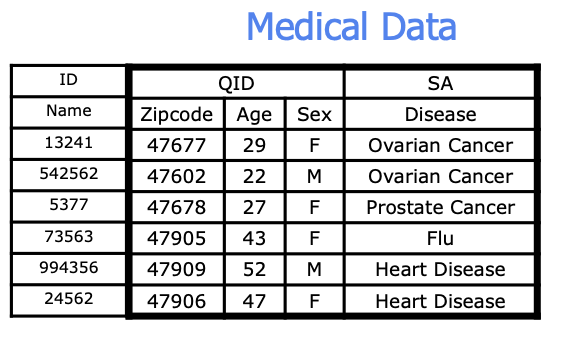
\includegraphics[width=0.3\textwidth]{medical-data}
    \label{fig:LABEL}
\end{figure}
\textcolor{red}{Possible existence of other databases (voter registration data)}

\begin{minipage}{0.4\textwidth}
% Quick centered image
\begin{figure}[H]
    \centering
    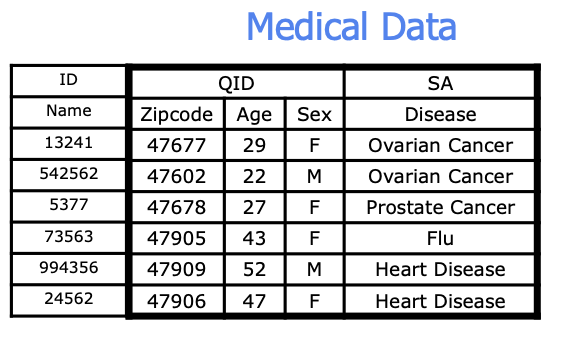
\includegraphics[width=0.8\textwidth]{medical-data}
    \label{fig:LABEL}
\end{figure}
\end{minipage}
\hfill
\begin{minipage}{0.35\textwidth}
\centering
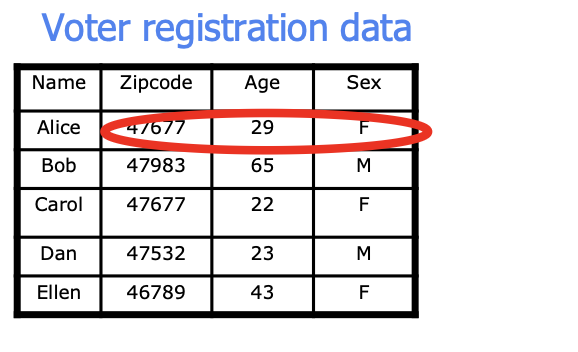
\includegraphics[width=\linewidth]{voter-data}
\end{minipage}

Let's remove identities

% Quick centered image
\begin{figure}[H]
    \centering
    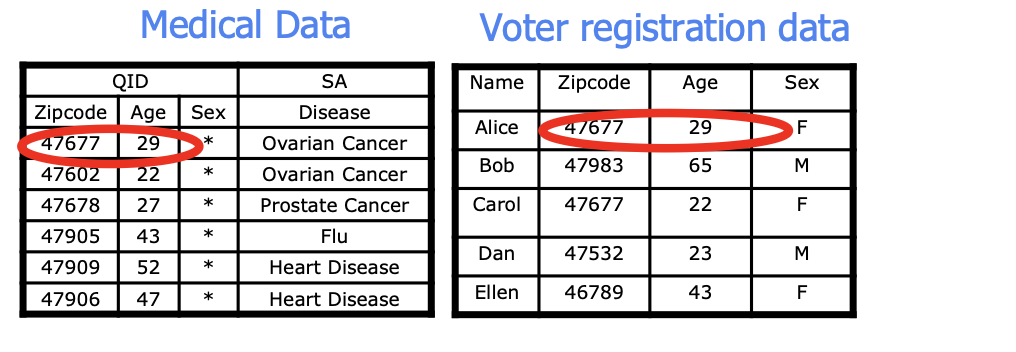
\includegraphics[width=0.5\textwidth]{identities-removed}
    \label{fig:LABEL}
\end{figure}
\textcolor{red}{some attributes are quasi-identifiers}

Let's remove some attributes

% Quick centered image
\begin{figure}[H]
    \centering
    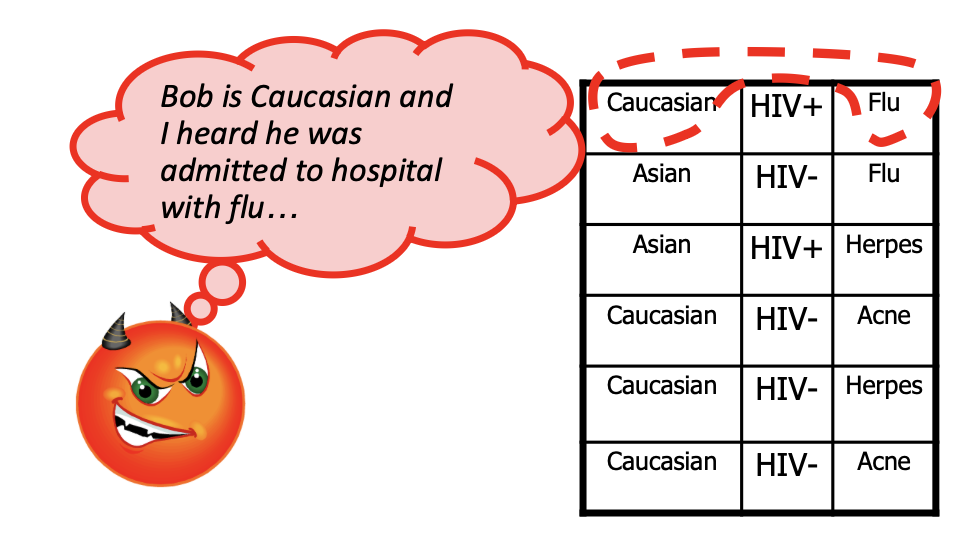
\includegraphics[width=0.35\textwidth]{attributes}
    \label{fig:LABEL}
\end{figure}

\textcolor{red}{Impossible to know what will be a QID}

\subsection*{k-anonymity}

\begin{minipage}{0.6\textwidth}
\begin{itemize}
	\item \textbf{Obfuscate QID} such that anonymity set for a user is at least k
	\item Each person contained in the database \textbf{cannot be distinguished from at least k-1 other individuals} whose information also appears in the released database
	\item k indicates the degree of anonymity
\end{itemize}

\end{minipage}
\hfill
\begin{minipage}{0.4\textwidth}
\centering
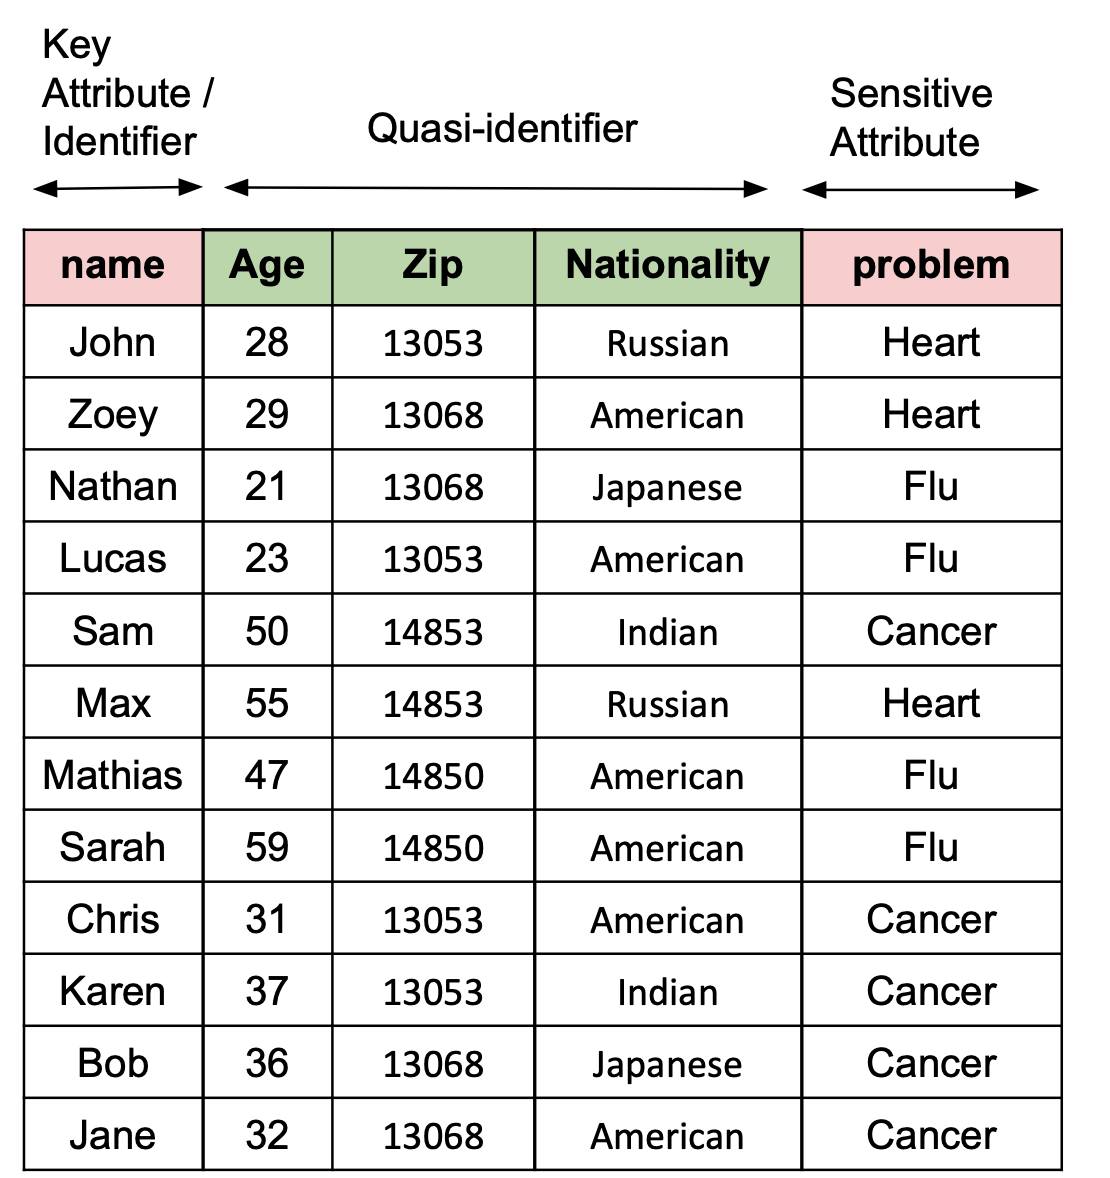
\includegraphics[width=\linewidth]{k-anonymity}
\end{minipage}

\begin{tcolorbox}[
  colback=blue!15,     % background color
  colframe=black!50,    % border color
  boxrule=1pt,       % border thickness
  arc=3mm,             % rounded corners
  left=4mm, right=4mm, top=2mm, bottom=2mm % padding
]
Equivalence class: group of records that are indistinguishable from QID
\end{tcolorbox}

% Quick centered image
\begin{figure}[H]
    \centering
    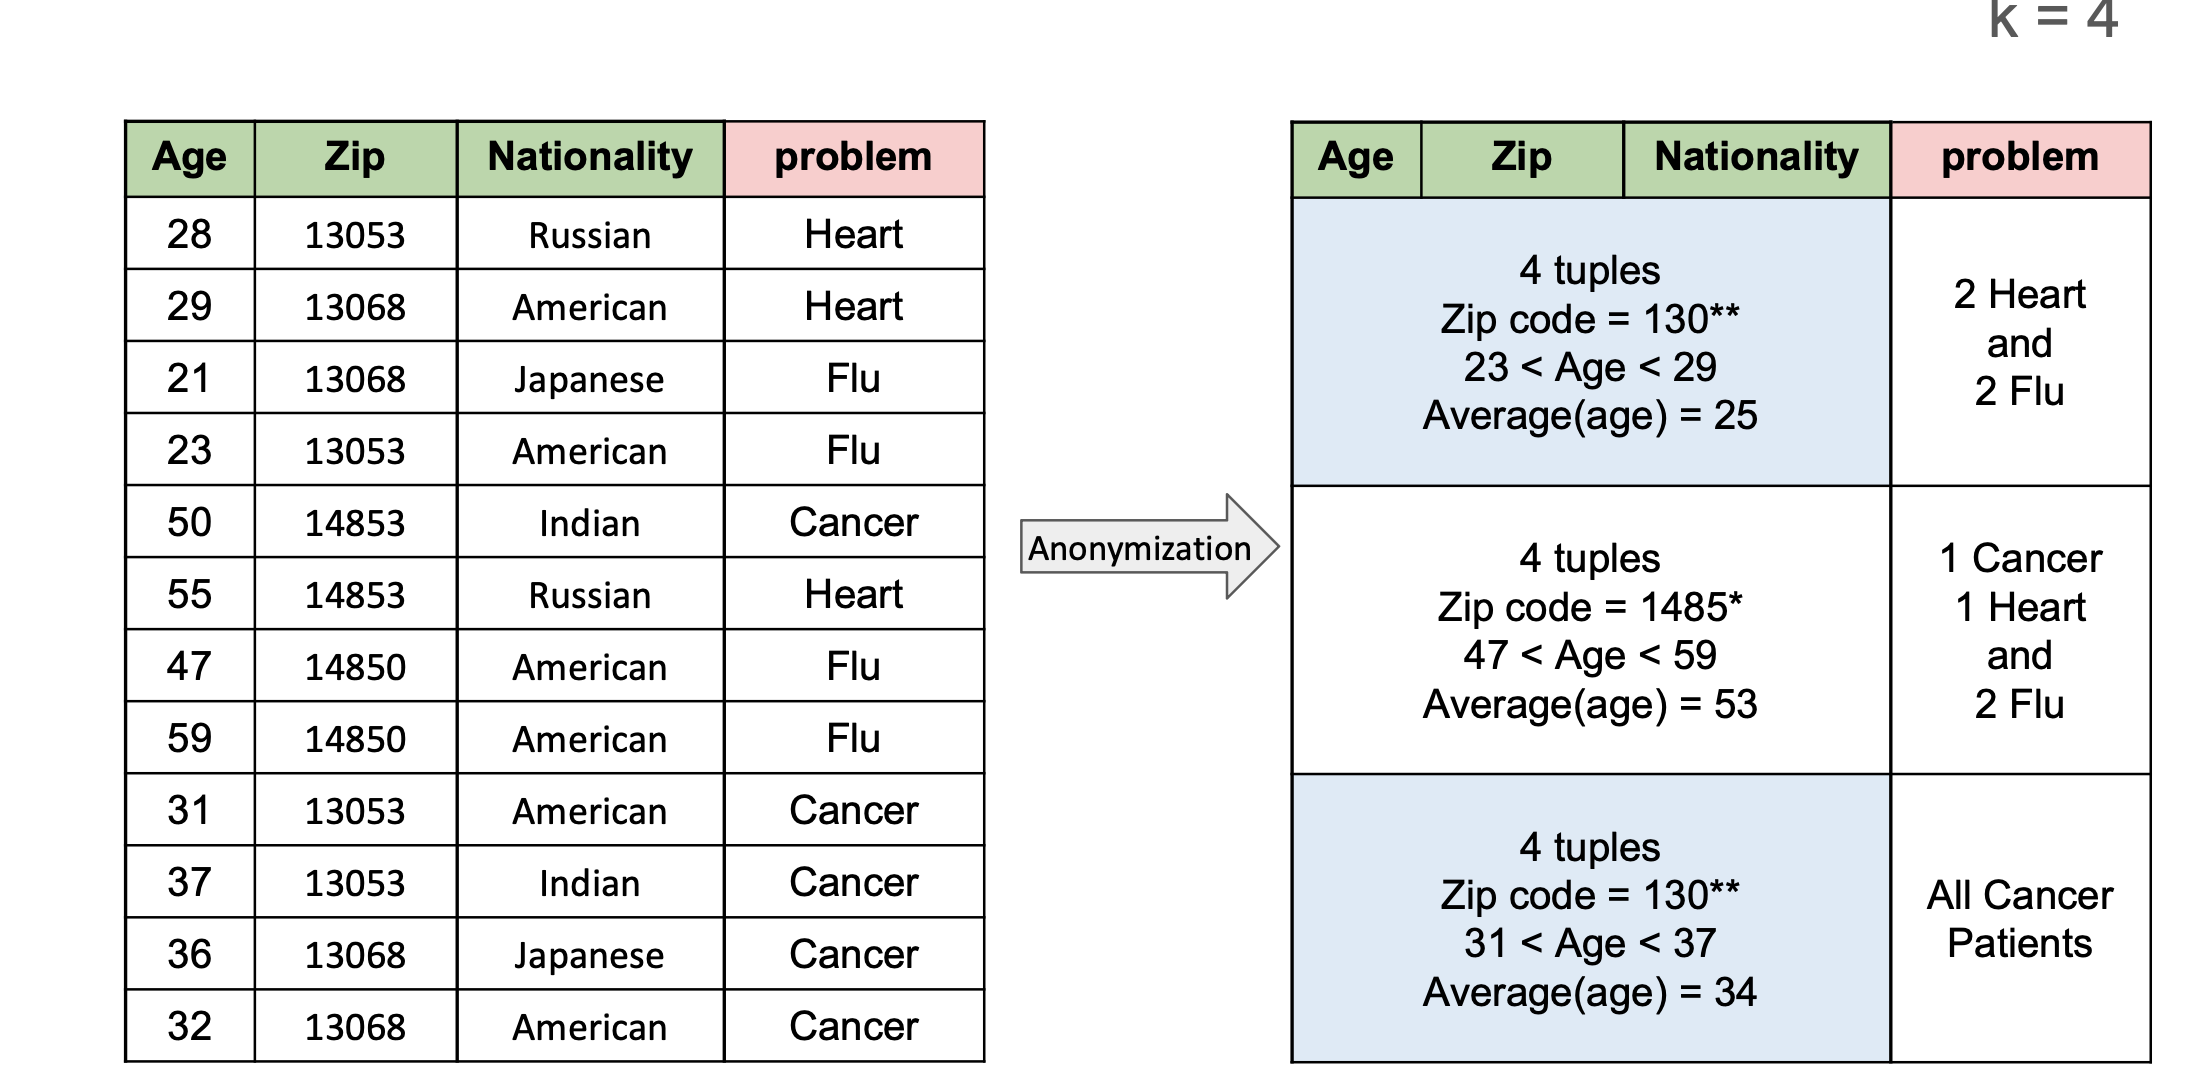
\includegraphics[width=0.8\textwidth]{k-4}
    \label{fig:LABEL}
\end{figure}

\begin{tcolorbox}[
  colback=\textcolor{red}{}!15,     % background color
  colframe=black!50,    % border color
  boxrule=1pt,       % border thickness
  arc=3mm,             % rounded corners
  left=4mm, right=4mm, top=2mm, bottom=2mm % padding
]
Homogeneity attack: in the third set all patients have cancer. Hence, it one knows Bob, his age and zip code, one can deduce information about the set. 
\end{tcolorbox}

\section*{L-Diversity}
\begin{tcolorbox}[
  colback=orange!15,     % background color
  colframe=black!50,    % border color
  boxrule=1pt,       % border thickness
  arc=3mm,             % rounded corners
  left=4mm, right=4mm, top=2mm, bottom=2mm % padding
]
Goal: preserve privacy by reducing granularity of data, extension of k-anonymity
\end{tcolorbox}
\begin{itemize}
	\item An equivalence class has $l$-diversity if there are at least  \textbf{$l$ well-presented values for the sensitive attribute}.
	\item A database has $l$-diversity if every equivalence class has $l$-diversity
\end{itemize}

\begin{tcolorbox}[
  colback=green!15,     % background color
  colframe=black!50,    % border color
  boxrule=1pt,       % border thickness
  arc=3mm,             % rounded corners
  left=4mm, right=4mm, top=2mm, bottom=2mm % padding
]
\textbf{In the previous table...}

\vspace{0.3cm}

3-diverse table: there are (at least) 3 different sensitive conditions in each equivalence class
\end{tcolorbox}

\subsection*{L-Diversity: Limitations}

% Quick centered image
\begin{figure}[H]
    \centering
    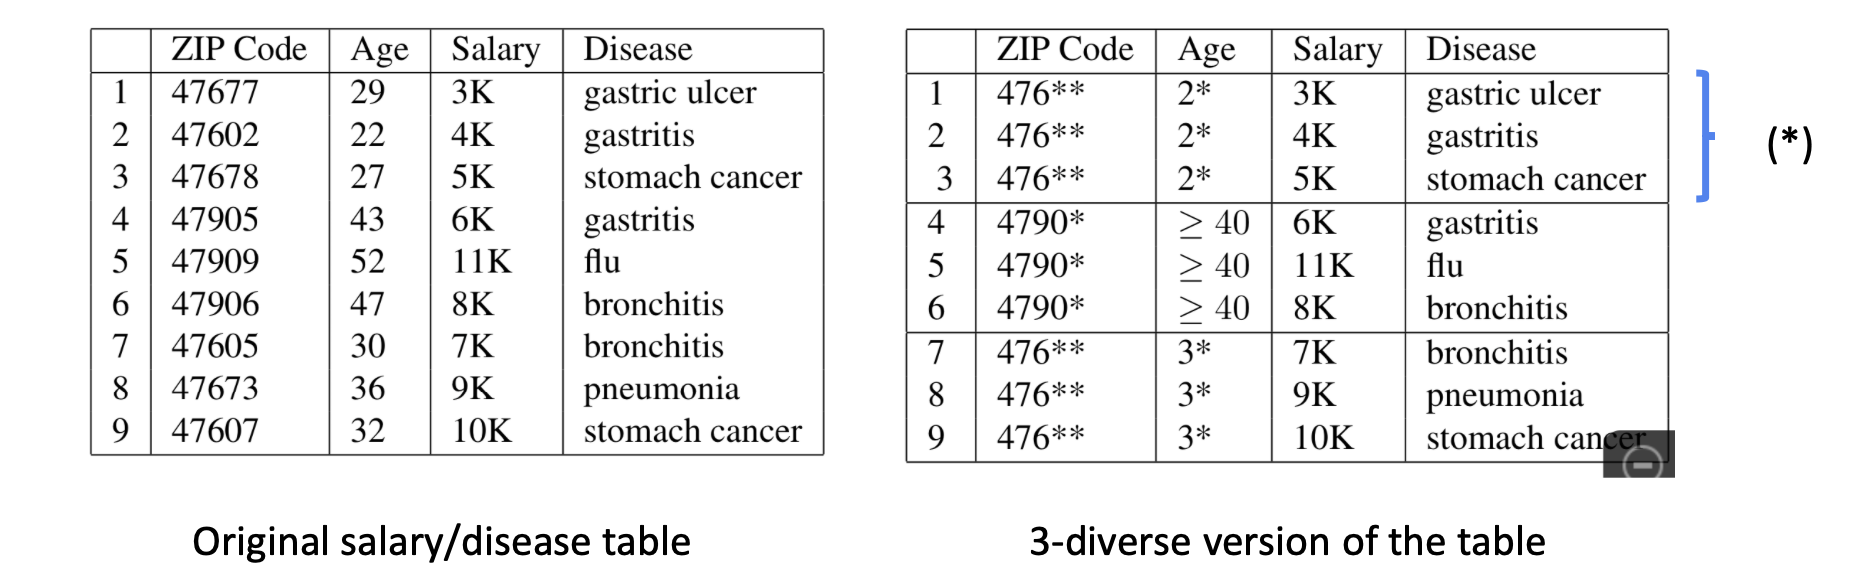
\includegraphics[width=0.8\textwidth]{l-limitations}
    \label{fig:LABEL}
\end{figure}

\begin{tcolorbox}[
  colback=red!15,     % background color
  colframe=black!50,    % border color
  boxrule=1pt,       % border thickness
  arc=3mm,             % rounded corners
  left=4mm, right=4mm, top=2mm, bottom=2mm % padding
]
Bob has a low income or is in his 20s, so he has a stomach-related disease. 
\end{tcolorbox}

\section*{t-closeness}
\begin{itemize}
	\item An equivalence class has \textbf{t-closeness if the distance between the distribution of a sensitive attribute in this class and the distribution of the attribute in the whole table is no more than a threshold t}
	\item A table has t-closeness if all equivalence classes have t-closeness.
	\item The distance is usually measured as earth mover's distance (EMD), also known as Wasserstein metric. 
\end{itemize}

\section*{Prior Knowledge Attack}

% Quick centered image
\begin{figure}[H]
    \centering
    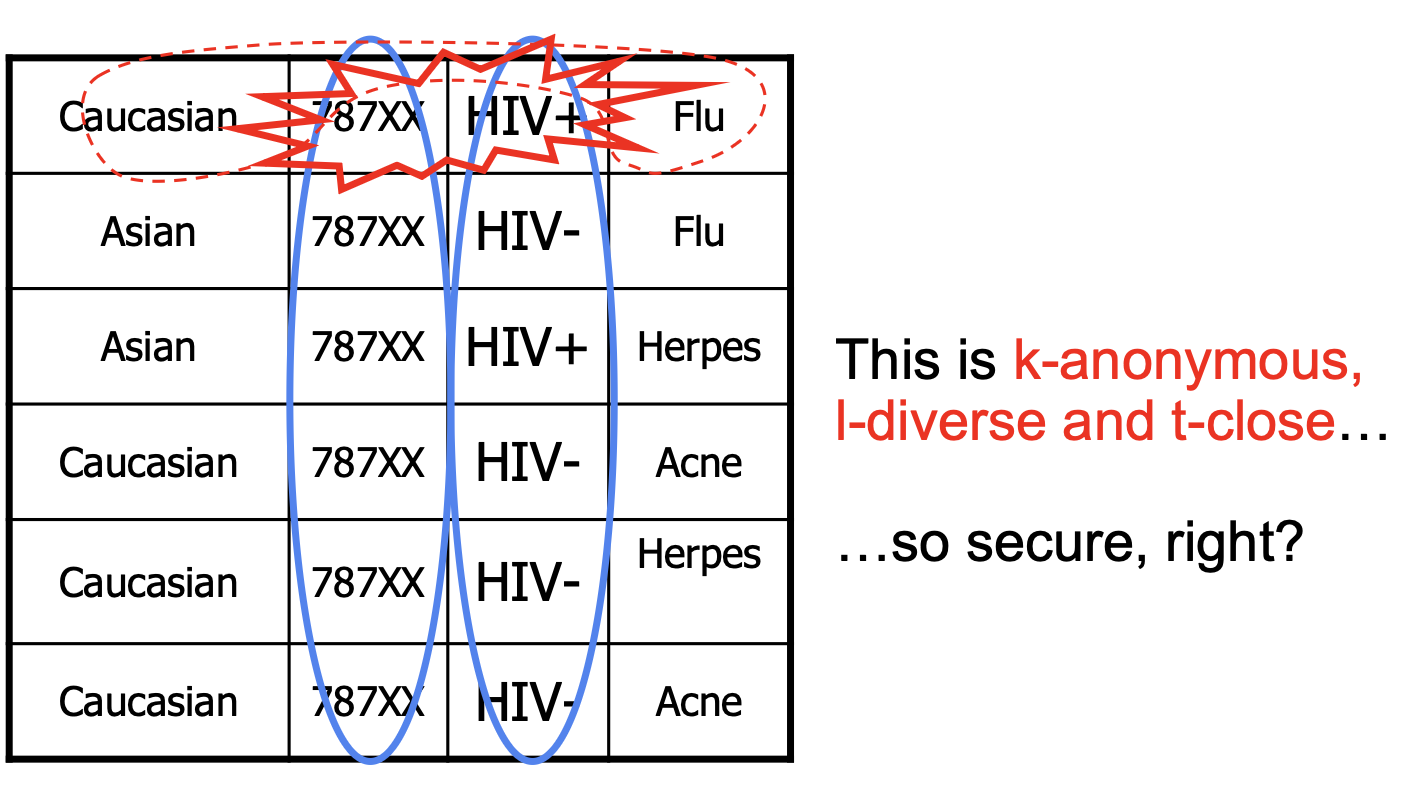
\includegraphics[width=0.6\textwidth]{prior-attack}
    \label{fig:LABEL}
\end{figure}

\begin{tcolorbox}[
  colback=red!15,     % background color
  colframe=black!50,    % border color
  boxrule=1pt,       % border thickness
  arc=3mm,             % rounded corners
  left=4mm, right=4mm, top=2mm, bottom=2mm % padding
]
Bob is Caucasian and I head he was admitted to hospital with flu...
\end{tcolorbox}

\newpage
\begin{center}
  {\LARGE \textbf{The Interactive Scenario}}
\end{center}
\vspace{0.5cm}

Many times we do not want the data, we want statistics!

\subsection*{Redefined Goal for the interactive case:}

Produce an \textbf{answer} that \textcolor{green}{preservers the utility} of the \textbf{statistics} \textcolor{red}{without leaking information} about individuals

% Quick centered image
\begin{figure}[H]
    \centering
    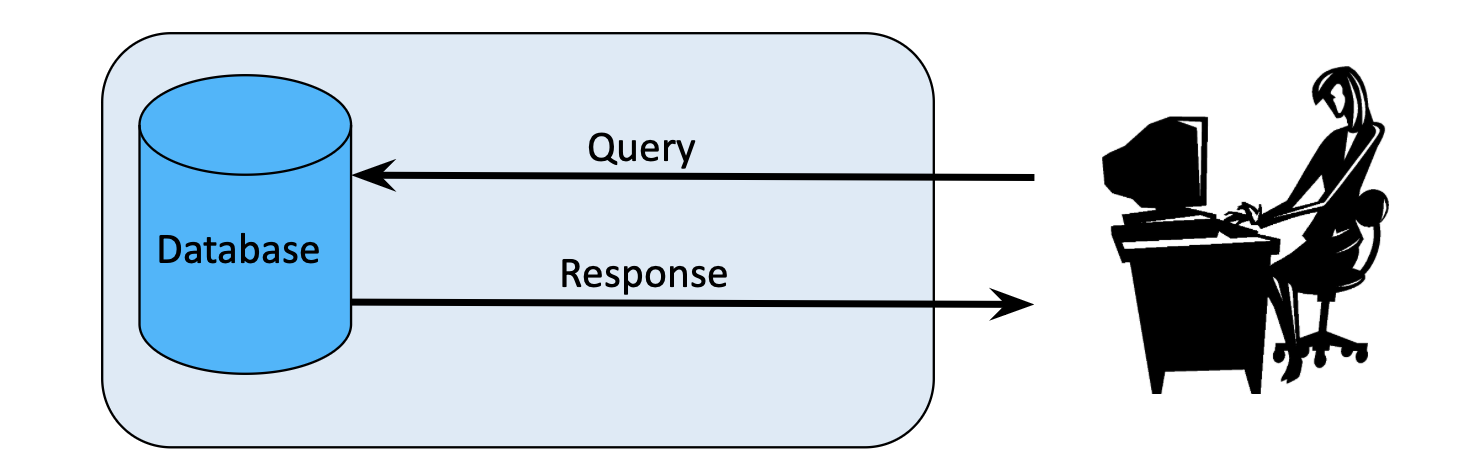
\includegraphics[width=0.7\textwidth]{interactive}
    \label{fig:LABEL}
\end{figure}

\textbf{Query:} What is the average salary of female professors at IC@EPFL with Greek nationality?

\textbf{\textcolor{red}{Is there a privacy problem?}}

The idea is to audit the queries, if the query will leak, deny! 

Either answer truthfully or state that where will be no answer. 

\textcolor{red}{Not answering already reveals some information!}

\subsection*{When denying fails: learning exact values}

Variables $d_i$ are real, privacy breached if adversary learns some  $d_i$

 % Quick centered image
\begin{figure}[H]
    \centering
    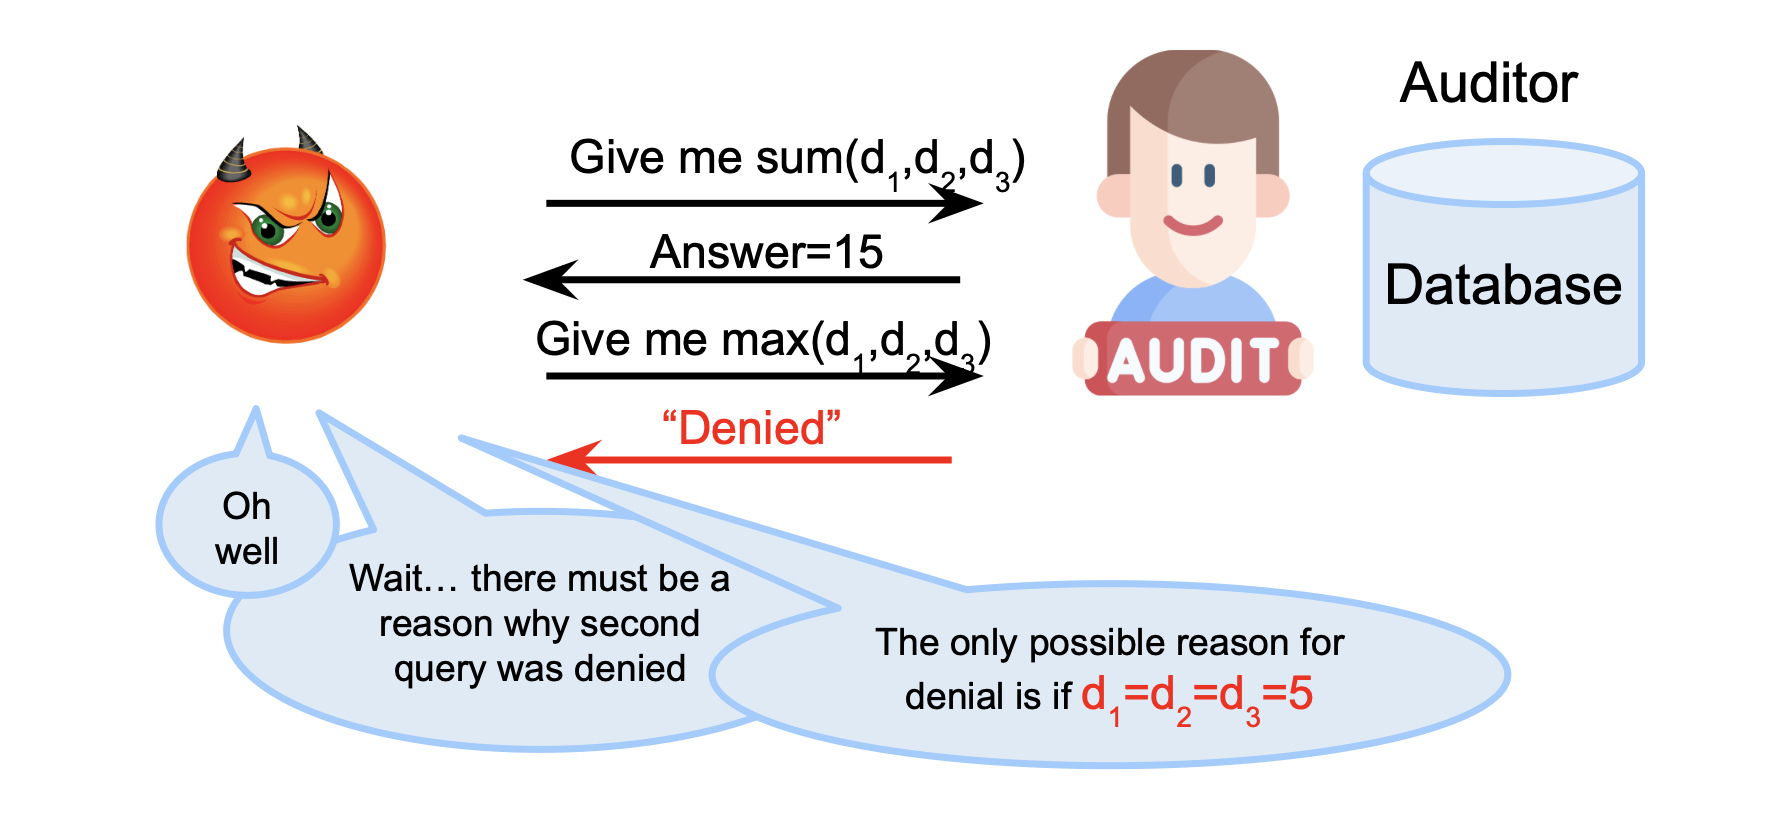
\includegraphics[width=0.6\textwidth]{denying-fails}
    \label{fig:LABEL}
\end{figure}

\subsection*{When denying fails: learning internals}

$d_i \in [0, 100]$, privacy breached if adversary learns some $d_i$ plus or minus 1

\section*{Auditing has problems}
\begin{itemize}
	\item Privacy definition? Privacy of Values? Groups? Exact?
	\item Algorithm limitations
		\begin{itemize}
			\item Secure deniability implies using algorithms computationally prohibitive
	\item Feasible focus mostly on simple queries
\end{itemize}
	\item Collusion? Either high cost or no security
	\item Utility?
		\begin{itemize}
			\item Percentage of denials may not be the best measure
		\end{itemize}
\end{itemize}

\vspace{0.5cm}

\begin{center}
  {\LARGE \textbf{Differential Privacy}}
\end{center}
\vspace{0.5cm}

\textbf{Remember the Goal for the interactive case}

\begin{itemize}
	\item Produce and \textbf{answer} that preserves the utility of statistics without leaking information about individuals
	\item To have any utility \textcolor{blue}{we must allow the leakage of some information}, but we can \textcolor{red}{set a bound of the extent of leakage}
	\item \textbf{\underline{Differential Privacy}}: Output is similar whether any single individual's record is included in the database or not.
\end{itemize}

\begin{itemize}
	\item \textbf{Basic philosophy}: instead of the real answer to a querry, add random noise to output, such that by a \textcolor{blue}{small change in the database (someone joins or leaves), the distribution of the answer does not change much}
	\item \textbf{A new privacy goal}: \textcolor{blue}{minimize the increased risk} incurred by an individual when joining (or leaving) a given database
	\item Differential Privacy is a privacy notion \textbf{NOT} a meachanism $\Rightarrow$ We use mechanisms to  \textit{achieve} differential privacy (e.g., add random noise)
\end{itemize}

\subsection*{Informal Definition}

Output is similar whether any single individual’s record is included in the database or not.

Records’s inclusion  in the computation does not make it \textit{significantly} \textcolor{red}{worse off}.

\begin{tcolorbox}[
  colback=blue!15,     % background color
  colframe=black!50,    % border color
  boxrule=1pt,       % border thickness
  arc=3mm,             % rounded corners
  left=4mm, right=4mm, top=2mm, bottom=2mm % padding
]
\textbf{If there is already some risk} of revealing a secret of a record by combining auxiliary information and something learned from DB, then \textbf{that risk is still there} but not \textit{significantly} increased by record's participation in the database.
\end{tcolorbox}

\subsection*{$\epsilon$-Differential Privacy - Format Definition}

An algorithm A satisfies $\epsilon$-diffrential privacy if
 \begin{itemize}
	 \item For \textbf{every pair or neighboring databases} ($D$, $D_{-r}$, differing only in row r)
	\item For \textbf{every subset S} of \textbf{possible output values} taken by A 
\end{itemize}
\[
	Pr[A(D) \in S] \leq e^{\epsilon} \times Pr[A(D_{-r}) \in S]
.\] 

\begin{tcolorbox}[
  colback=green!15,     % background color
  colframe=black!50,    % border color
  boxrule=1pt,       % border thickness
  arc=3mm,             % rounded corners
  left=4mm, right=4mm, top=2mm, bottom=2mm % padding
]
\underline{Principle}: The \textbf{removal/addition} of a \textbf{single record} in the \textbf{database should/does not substantially affect the values} of the computed function/statistics. 
\end{tcolorbox}

\subsection*{Properties of Differential Privacy}

\begin{itemize}
	\item \textbf{Composability: If algorithms $A_1$, $A_2$, ..., $A_k$} \textcolor{blue}{use independent randomness} and \textcolor{blue}{each \textbf{$A_i$} satisfies $\epsilon_i$-differential privacy}, respectively. Then ($A_1$, $A_2$, ..., $A_k$) is \textbf{($\epsilon_1$ + $\epsilon_2$ + ... + $\epsilon_k$)-differentially private}
	\item \textbf{Post-processing secure}: If algorithms A is $\epsilon$-differentially private, then \textcolor{blue}{for all functions g}, g(A) is also $\epsilon$-differentially private  \textcolor{blue}{(cannot undo privacy with more computations)}
\end{itemize}

\section*{How to ensure differentially privacy?}

\begin{itemize}
	\item \textbf{Input pertubation}
		\begin{itemize}
			\item Add noise directly to the database (\textcolor{red}{$\neq$} perturbed database can be published) \\
			\textcolor{green}{+} independent of the algorithm \textcolor{green}{and} easy to reproduce \\
			\textcolor{red}{-} determing the amount of required noise is difficult
		\end{itemize}
	\item \textbf{Output perturbation}
		\begin{itemize}
			\item Add noise to the function (statistic) output \\
				\textcolor{green}{+} easier to control privacy \textcolor{green}{and} better guarantees than input perturbation \\
				\textcolor{red}{-} results cannot be reproduced
		\end{itemize}
	\item \textbf{Algorithm Perturbation}
		\begin{itemize}
			\item Inherently add noise to the algo \\
			\textcolor{green}{+} algorithm can be optimized with the noise addition \\
			\textcolor{red}{-} difficult to generalize \textcolor{red}{and} depends on the inputs
		\end{itemize}
\end{itemize}


\section*{Differentialy privacy comes at a cost}
\begin{itemize}
	\item \textbf{Impact on accuracy}: we still add noise!
	\item \textbf{Impact is disparate}: we preserve the average signal... but not the outliers
	\item \textbf{Very hard to implement in practice}: sensitivity is not always obvious to compute, independence is not always guaranteed
\end{itemize}
\end{document}
